\documentclass[11pt]{asaproc}\usepackage[]{graphicx}\usepackage[]{color}
%% maxwidth is the original width if it is less than linewidth
%% otherwise use linewidth (to make sure the graphics do not exceed the margin)
\makeatletter
\def\maxwidth{ %
  \ifdim\Gin@nat@width>\linewidth
    \linewidth
  \else
    \Gin@nat@width
  \fi
}
\makeatother

\definecolor{fgcolor}{rgb}{0.345, 0.345, 0.345}
\newcommand{\hlnum}[1]{\textcolor[rgb]{0.686,0.059,0.569}{#1}}%
\newcommand{\hlstr}[1]{\textcolor[rgb]{0.192,0.494,0.8}{#1}}%
\newcommand{\hlcom}[1]{\textcolor[rgb]{0.678,0.584,0.686}{\textit{#1}}}%
\newcommand{\hlopt}[1]{\textcolor[rgb]{0,0,0}{#1}}%
\newcommand{\hlstd}[1]{\textcolor[rgb]{0.345,0.345,0.345}{#1}}%
\newcommand{\hlkwa}[1]{\textcolor[rgb]{0.161,0.373,0.58}{\textbf{#1}}}%
\newcommand{\hlkwb}[1]{\textcolor[rgb]{0.69,0.353,0.396}{#1}}%
\newcommand{\hlkwc}[1]{\textcolor[rgb]{0.333,0.667,0.333}{#1}}%
\newcommand{\hlkwd}[1]{\textcolor[rgb]{0.737,0.353,0.396}{\textbf{#1}}}%
\let\hlipl\hlkwb

\usepackage{framed}
\makeatletter
\newenvironment{kframe}{%
 \def\at@end@of@kframe{}%
 \ifinner\ifhmode%
  \def\at@end@of@kframe{\end{minipage}}%
  \begin{minipage}{\columnwidth}%
 \fi\fi%
 \def\FrameCommand##1{\hskip\@totalleftmargin \hskip-\fboxsep
 \colorbox{shadecolor}{##1}\hskip-\fboxsep
     % There is no \\@totalrightmargin, so:
     \hskip-\linewidth \hskip-\@totalleftmargin \hskip\columnwidth}%
 \MakeFramed {\advance\hsize-\width
   \@totalleftmargin\z@ \linewidth\hsize
   \@setminipage}}%
 {\par\unskip\endMakeFramed%
 \at@end@of@kframe}
\makeatother

\definecolor{shadecolor}{rgb}{.97, .97, .97}
\definecolor{messagecolor}{rgb}{0, 0, 0}
\definecolor{warningcolor}{rgb}{1, 0, 1}
\definecolor{errorcolor}{rgb}{1, 0, 0}
\newenvironment{knitrout}{}{} % an empty environment to be redefined in TeX

\usepackage{alltt}

\usepackage{graphicx}
\usepackage{natbib}
\usepackage[hyphens]{url}
\usepackage{color}
\usepackage{times}
\usepackage{verbatim}
%\usepackage{enumitem}
\usepackage[hidelinks,breaklinks=true]{hyperref}


\renewcommand\labelenumi{(\roman{enumi})}
\renewcommand\theenumi\labelenumi

\title{An Interactive Tool to Visualize Results from Uncertainty Quantification}

\author{Matthew Isaac \thanks{Department of Mathematics and Statistics, Utah State University, Logan, UT 84322--3900, USA. 
E-mail: \url{matt.isaac@aggiemail.usu.edu}}
}
\IfFileExists{upquote.sty}{\usepackage{upquote}}{}
\begin{document}

\renewcommand{\topfraction}{1.0}
\renewcommand{\bottomfraction}{1.0}
\renewcommand{\textfraction}{0.0}
\renewcommand{\floatpagefraction}{1.0}
\renewcommand{\dbltopfraction}{1.0}


\maketitle

\begin{abstract}
Uncertainty quantification is a class of methods used to simulate the ways that variations to inputs of a system can potentially change the end state of that system. This paper outlines the implementation of an interactive tool to visualize the results of an uncertainty quantification analysis. The interactive tool is a deployable web application built with the {\tt R Shiny} framework. Users can create, adjust, and save custom visualizations to assist in interpreting and presenting results. 
\end{abstract}

\begin{keywords}Uncertainty Quantification; Statistical Visualization; Interactive Visualization; {\tt shiny} R Package
\end{keywords}


%%%%%%%%%%%%%%%%%%%%%%%%%
\section{Introduction}
\label{Introduction}
%%%%%%%%%%%%%%%%%%%%%%%%%

Uncertainty quantification is a methodological framework used with some frequency in engineering analysis \citep{EW2018}. It is used to understand how variability  within the parameters (i.e. inputs) to some system impact the end state of that system. Engineering analysts use uncertainty quantification to assess and find the balance between design sufficiency and design efficiency. This is particularly important in fields where large-scale prototypes, testing, and data collection are extremely expensive. Engineers in these types of applications are increasingly relying on computational simulations to assess system designs.

In the following paper, I outline the implementation of an interactive tool to visualize uncertainty quantification results. The outline of this paper will proceed as follows: In Section~\ref{UQOverview}, a brief overview of uncertainty quantification is given. In Section~\ref{Methods}, the methods by which the visualization tool was developed are described. In Section~\ref{Results}, the resulting web application is described and screenshots of the web application are shown. In Section~\ref{Future}, future enhancements to the web application are discussed. Section~\ref{Appendix} contains the code written to generate the {\tt shiny} app.

%%%%%%%%%%%%%%%%%%%%%%%%%
\section{Uncertainty Quantification Overview}  
\label{UQOverview}
%%%%%%%%%%%%%%%%%%%%%%%%%

The following description of the uncertainty quantification algorithm is adapted from \cite{EW2018}. First, a few terms and definitions will be described. 

\begin{description}
\item[system response quantity (SRQ):] A parameter of particular interest directly related to the engineering system in question. The SRQ is the output (i.e. prediction) from the engineering model.
\item[engineering model:] A mathematical model that defines the relationship between the parameters (model inputs) and SRQ (model output). 
\item[aleatory uncertainty:] Uncertainty resulting from randomness inherent to a given parameter. Gaining more knowledge about the parameter will not reduce the uncertainty of the parameter. 
\item[epistemic uncertainty:] Uncertainty resulting from a lack of knowledge about a given parameter. Gaining more knowledge about the parameter could reduce the uncertainty of the parameter. 
\end{description}

The first step of uncertainty quantification is to identify sources of uncertainty (model parameters) and classify them as either aleatory or epistemic. This classification process has been somewhate debated in literature \citep{KD2009}, and will not be discussed as it is outside the scope of this project. Once these uncertainties related to the model parameters have been identified and classified as aleatory or epistemic, the uncertainty for each parameter must somehow be described. Traditionally, epistemic uncertainties have been described by an interval over which any value in the interval is equally likely, while aleatory uncertainties have been assigned probability distributions. Some more recent publications \citep{EW2018} propose that all uncertainties, aleatory or epistemic, be described using probability distributions. This debate will not be discussed here as it is, again, outside the scope of this project. Once these distributions and/or intervals have all been assigned, they are carried through the model using Monte Carlo techniques.

Let $m$ denote the number of iterations of an outer for loop, and let $n$ denote the number of iterations in an inner for loop. In the outer for loop, values for the epistemic uncertainty parameters are selected randomly from the intervals/distributions assigned. Upon entering the inner loop, values for the aleatory uncertainty parameters are randomly chosen from the distributions assigned. The values chosen for the parameters in both the outer loop and the inner loop are then used as inputs in the engineering model to calculate a value for the SRQ. This value is stored and the inner loop continues running for the rest of the $n-1$ iterations. All of the $n$ SRQ values calculated from the $n$ iterations of the inner loop are used to calculate an empirical cumulative distribution function (CDF) of SRQ values and the CDF is stored. The outer loop then begins its second iteration, and new values for the empirical uncertainty parameters are chosen. The inner loop then runs another $n$ iterations, producing another CDF. This process continues until the outer loop has run all of its $m$ iterations. 

At this point, there will be $m$ empirical CDFs that have been calculated, representing various possible realized values of the SRQ. These CDFs can then be plotted and interpreted. \cite{EW2018} suggests constructing a ``P-box". This P-box is found by calculating a lower percentile (e.g. the 5th percentile) and an upper percentile (e.g. the 95th percentile) of the CDF ensemble. This P-box can then be interpreted in several ways, including (1) selecting a SRQ value and extracting a probability interval, and (2) selecting a probability value and extracting an SRQ interval.

%%%%%%%%%%%%%%%%%%%%%%%%%
\section{Methods}  
\label{Methods}
%%%%%%%%%%%%%%%%%%%%%%%%%

In order to assist analysts in visualizing and interpreting results from an uncertainty quantification analysis as described in Section~\ref{UQOverview}, an interactive visualization tool was developed. Since the actual uncertainty quantification analysis can be carried out with greater speed and computational power elsewhere, this implementation does not include the Monte Carlo portion of the implementation described in Section~\ref{UQOverview}. The web application was built using the {\tt shiny R} package and the code for this application is contained in two files. The first file, {\tt ui.R} (short for `user interface') contains the code that controls the layout of the various panels and panes in the application, as well as the placement of the user interface elements (i.e. text inputs, sliders, etc.). The {\tt server.R} file contains the computational code that performs calculations, data manipulation, and generates the plots. See Section~\ref{Appendix} for the source code. 

\subsection{{\tt R} Packages}
The following packages and methods were used in the development of the web application:

\begin{description}

\item[{\bf dplyr:}] The {\tt dplyr} package \citep{DPLYR} is a data-wrangling and manipulation package implemented in {\tt R}. The methods in this package were used to manage and manipulate the CDFs from the {\tt .csv} file into a convenient format for plotting. 

\item[{\bf shiny:}] The {\tt shiny} package and framework \citep{SHINY} constitues the backbone of this project. {\tt shiny} provides a way to create and deploy web applications through RStudio \citep{RSTUDIO}. It also contains the implementations for all user-interface components (toggle buttons, check boxes, numeric inputs, sliders, etc.). The {\tt shinydashboard} package \citep{DASH} was also used as an aesthetic wrapper around the {\tt shiny} framework. The {\tt shiny} package was be used to create and will be used to deploy the web application.

\item[{\bf ggplot2:}] The plotting functionality of the {\tt ggplot2} package \citep{GGPLOT} was used to generate the actual visualization and to add, remove, or adjust components on the plot. 

\item[{\bf plotly:}] The {\tt plotly} package \citep{PLOTLY} is not currently used in the implementation, but may be used to add additional interactive capabilities to the plot. {\tt plotly} includes a method called {\tt ggplotly()} which could be used to convert the {\tt ggplot} plot object to a {\tt plotly} plot object. The {\tt plotly} plots contain options to zoom in and out on a plot, show plot values when hovering with mouse, download and save a {\tt .png} version of the plot, and download and save an interactive {\tt html} version of the plot. 
\end{description}

\vspace{5mm}

Since the existing {\tt R} packages already implemented most of the tools needed to generate the plot and implement user interface elements, the primary task on this project was to seamlessly combine elements from the packages above (particularly the {\tt shiny}, {\tt ggplot2}, and {\tt plotly} packages) to create a user-friendly interactive visualization tool. 

% \subsection{User Guide}
% Users begin by selecting a data source using toggle buttons, selecting either provided sample data, or uploading a {.csv} file. An uploaded {\tt .csv} file should contain the 'x' values (i.e. values of the SRQ that the CDf is evaluated over) in the first column and individual values of the CDFs in the rest of the columns. 

%%%%%%%%%%%%%%%%%%%%%%%%%
\section{Results}
\label{Results}
%%%%%%%%%%%%%%%%%%%%%%%%%

\subsection{Features}
The resulting web application currently has the several features implemented. First, the capability was added to allow the user to upload their own data from a {\tt .csv} file to be used in the visualization. If users want to experiment with the visualization but don't have their own data readily on hand, they can also choose to use some provided sample data.  Once the data source is specified by the user, several options are provided to allow customization of the visualization. Users can show or hide the P-box, as well as specify the upper and lower percentiles to be used in the P-box calculation. The CDF ensemble can also be toggled on and off so only the P-box is shown. Oftentimes there are hundreds or thousands of CDFs to be plotted, so naturally a lot of overplotting can occur. A slider is included in the control panel to adjust the tranparency of the CDFs. A download button has also been provided so users can download and save a {\tt .png} file of the current rendering of the plot. 

% \begin{itemize}
% \item experiment with provided sample data
% \item upload data from a {\tt .csv} file 
% \item toggle P-box on/off
% \item toggle CDF ensemble on/off
% \item select upper and lower percentiles to be used in P-box calculation
% \item select level of transparency for CDF ensemble
% \item download and save the visualization in its current state
% \item view user manual
% \end{itemize}

A few preliminary screenshots from the web application are included in this paper. Figure~\ref{dwnld_plt} shows downloaded plots with various plotting options selected (show/hide P-box and CDFs). Figure~\ref{full} shows a full-view screenshot of the application.  

\begin{figure}[t]
\begin{center} 
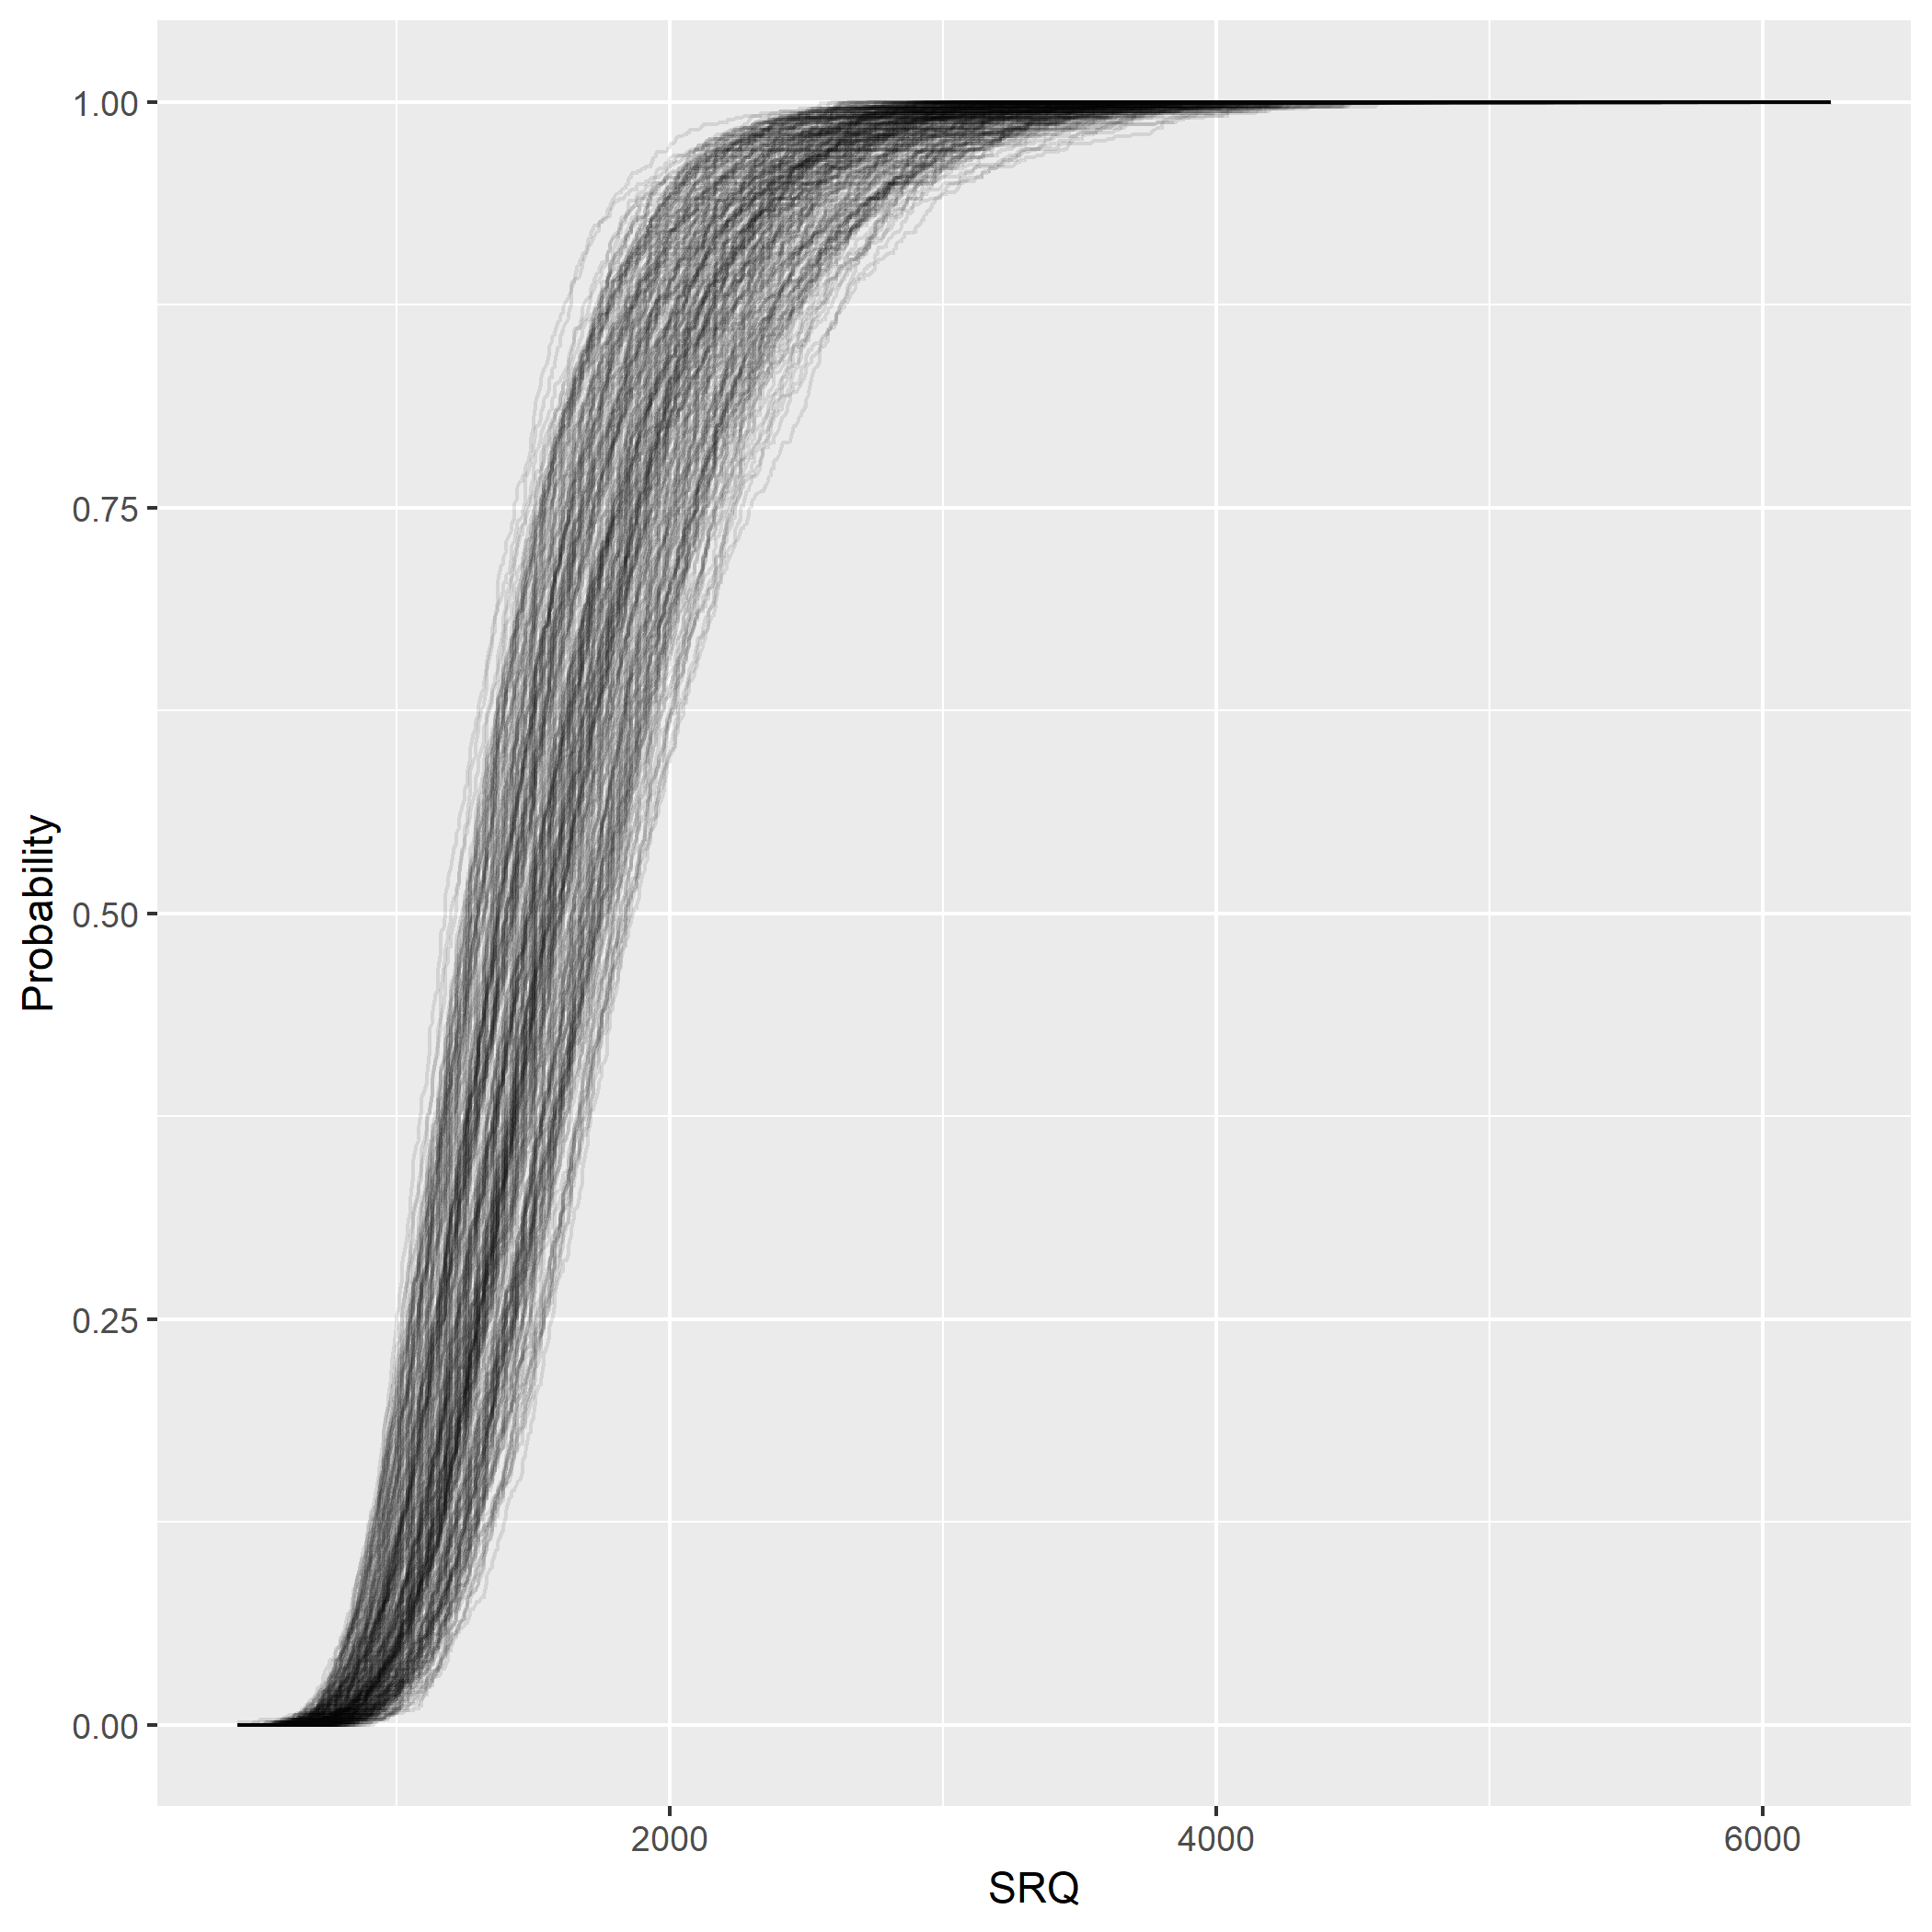
\includegraphics[height=4.3cm,width=4.3cm]{figures2/dwnld_plt_cdfs.png}
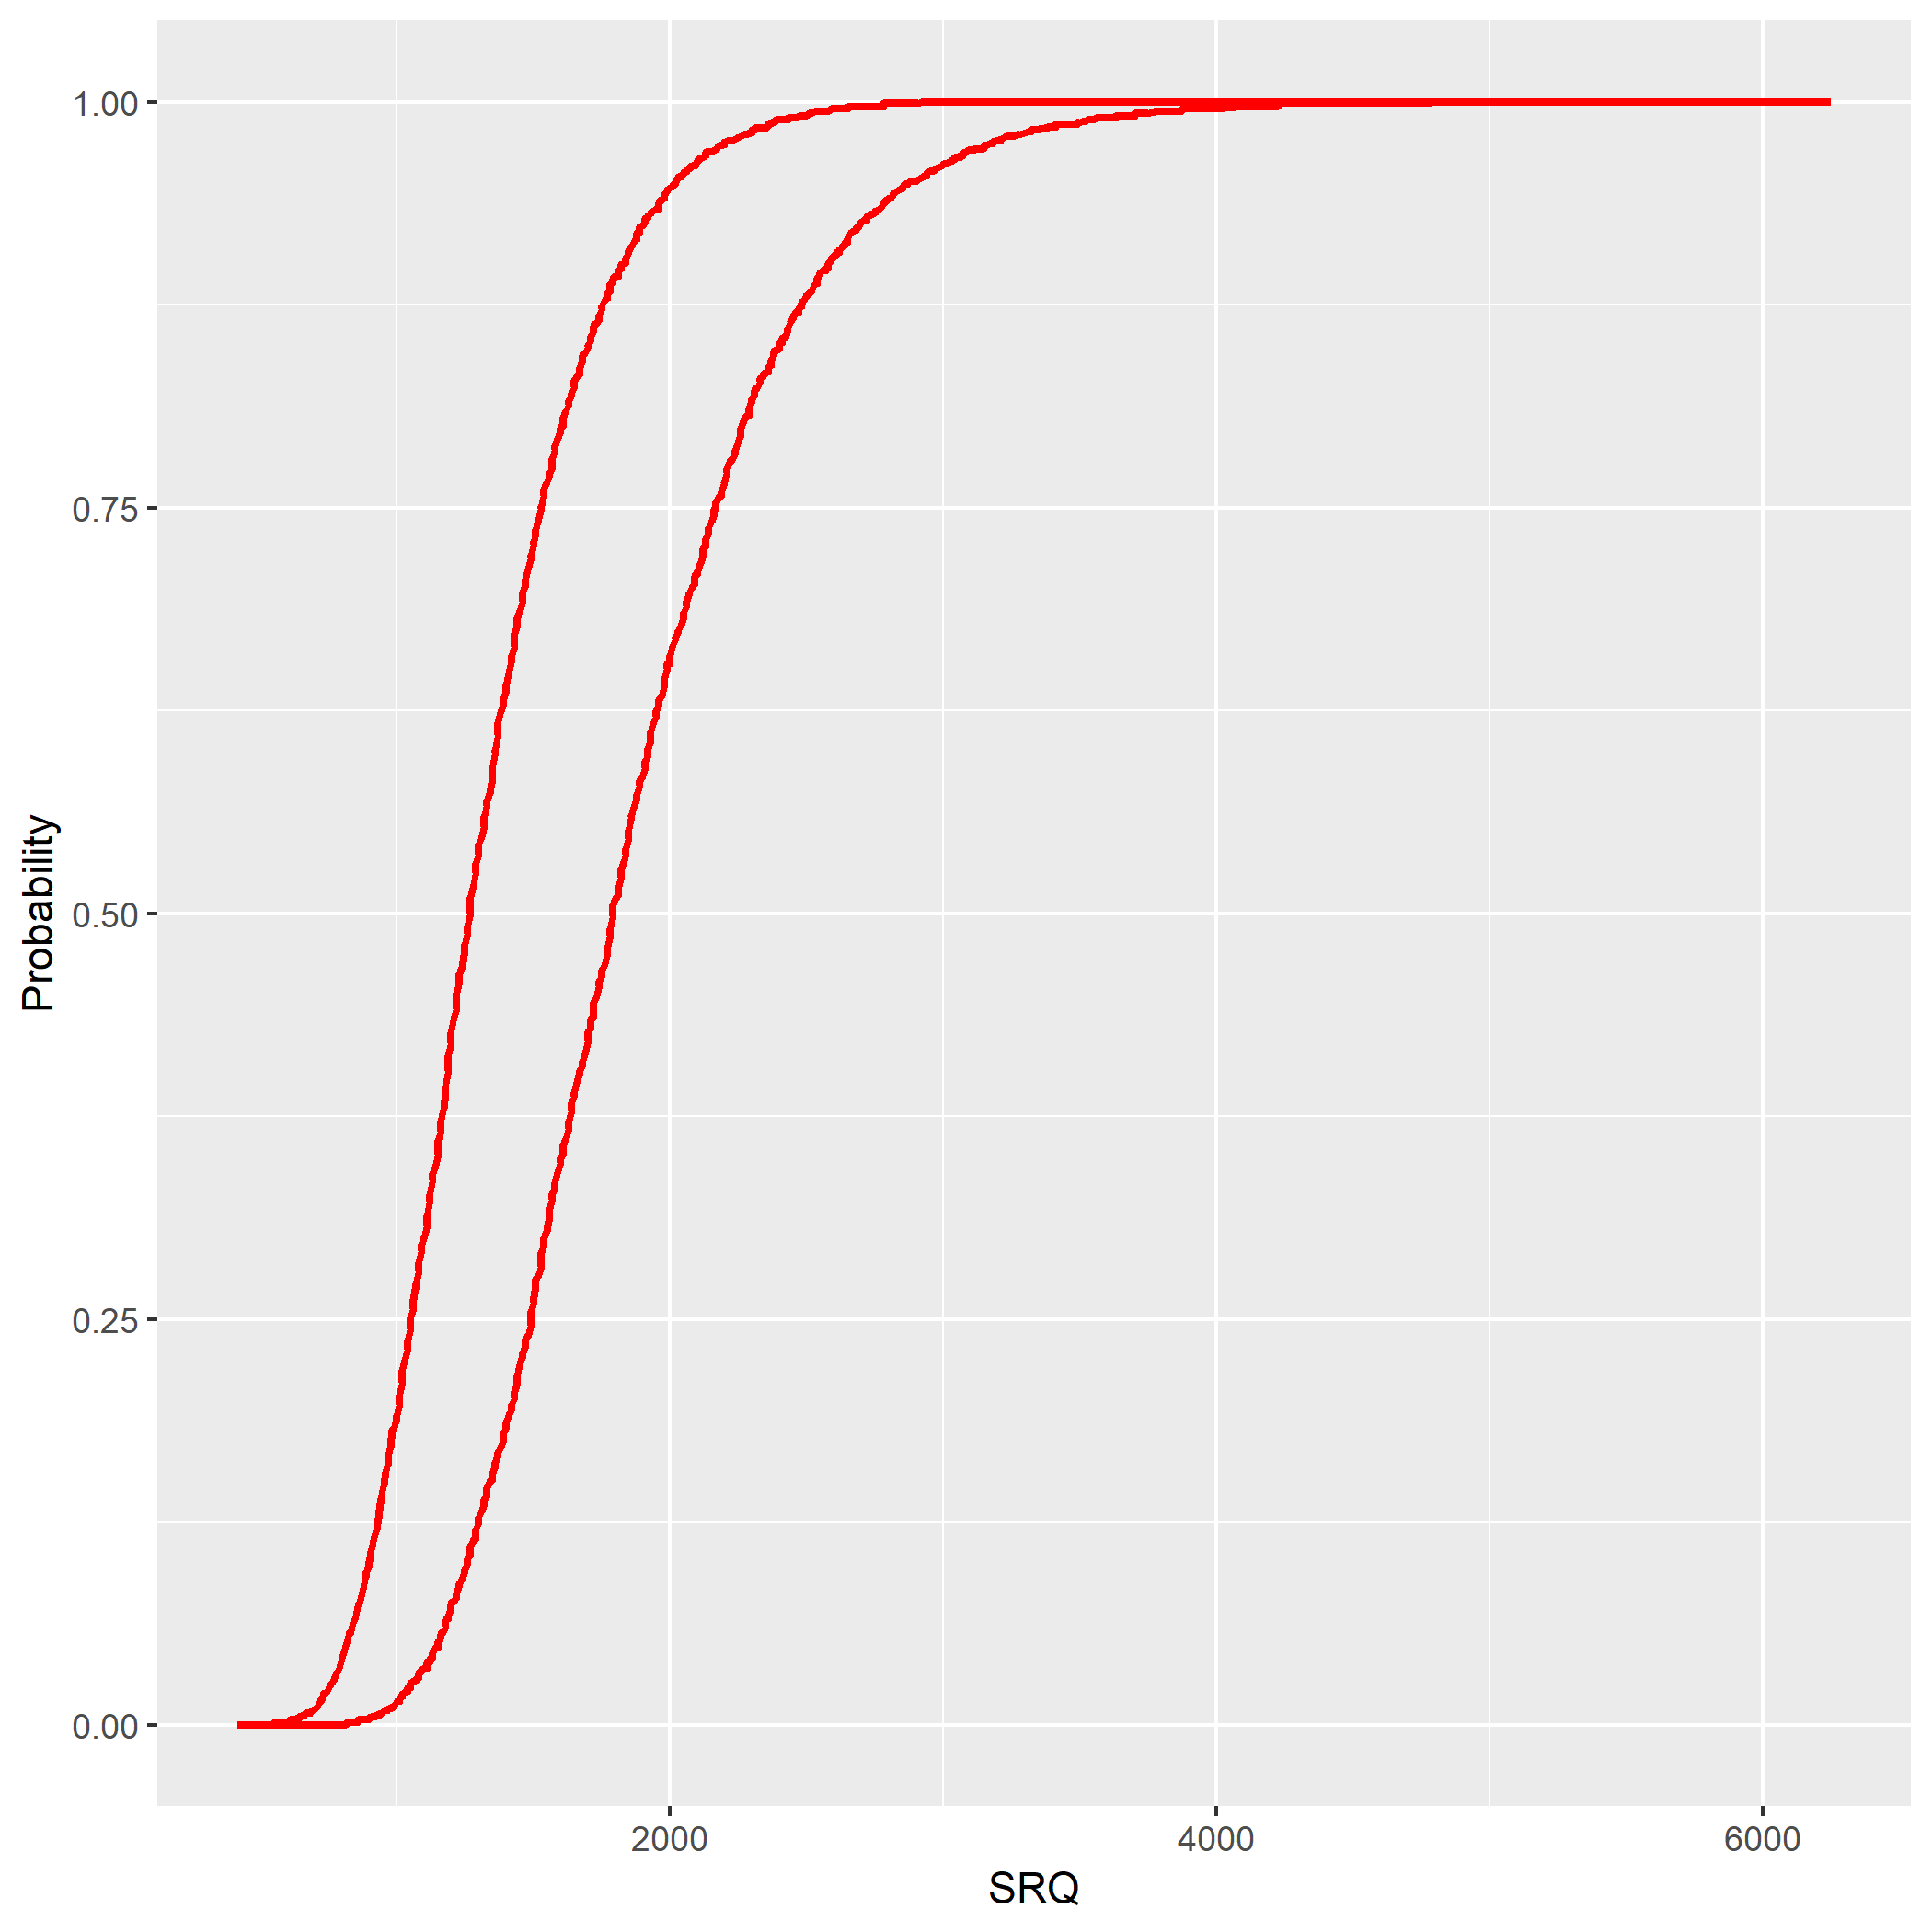
\includegraphics[height=4.3cm,width=4.3cm]{figures2/dwnld_plt_pbx.png}
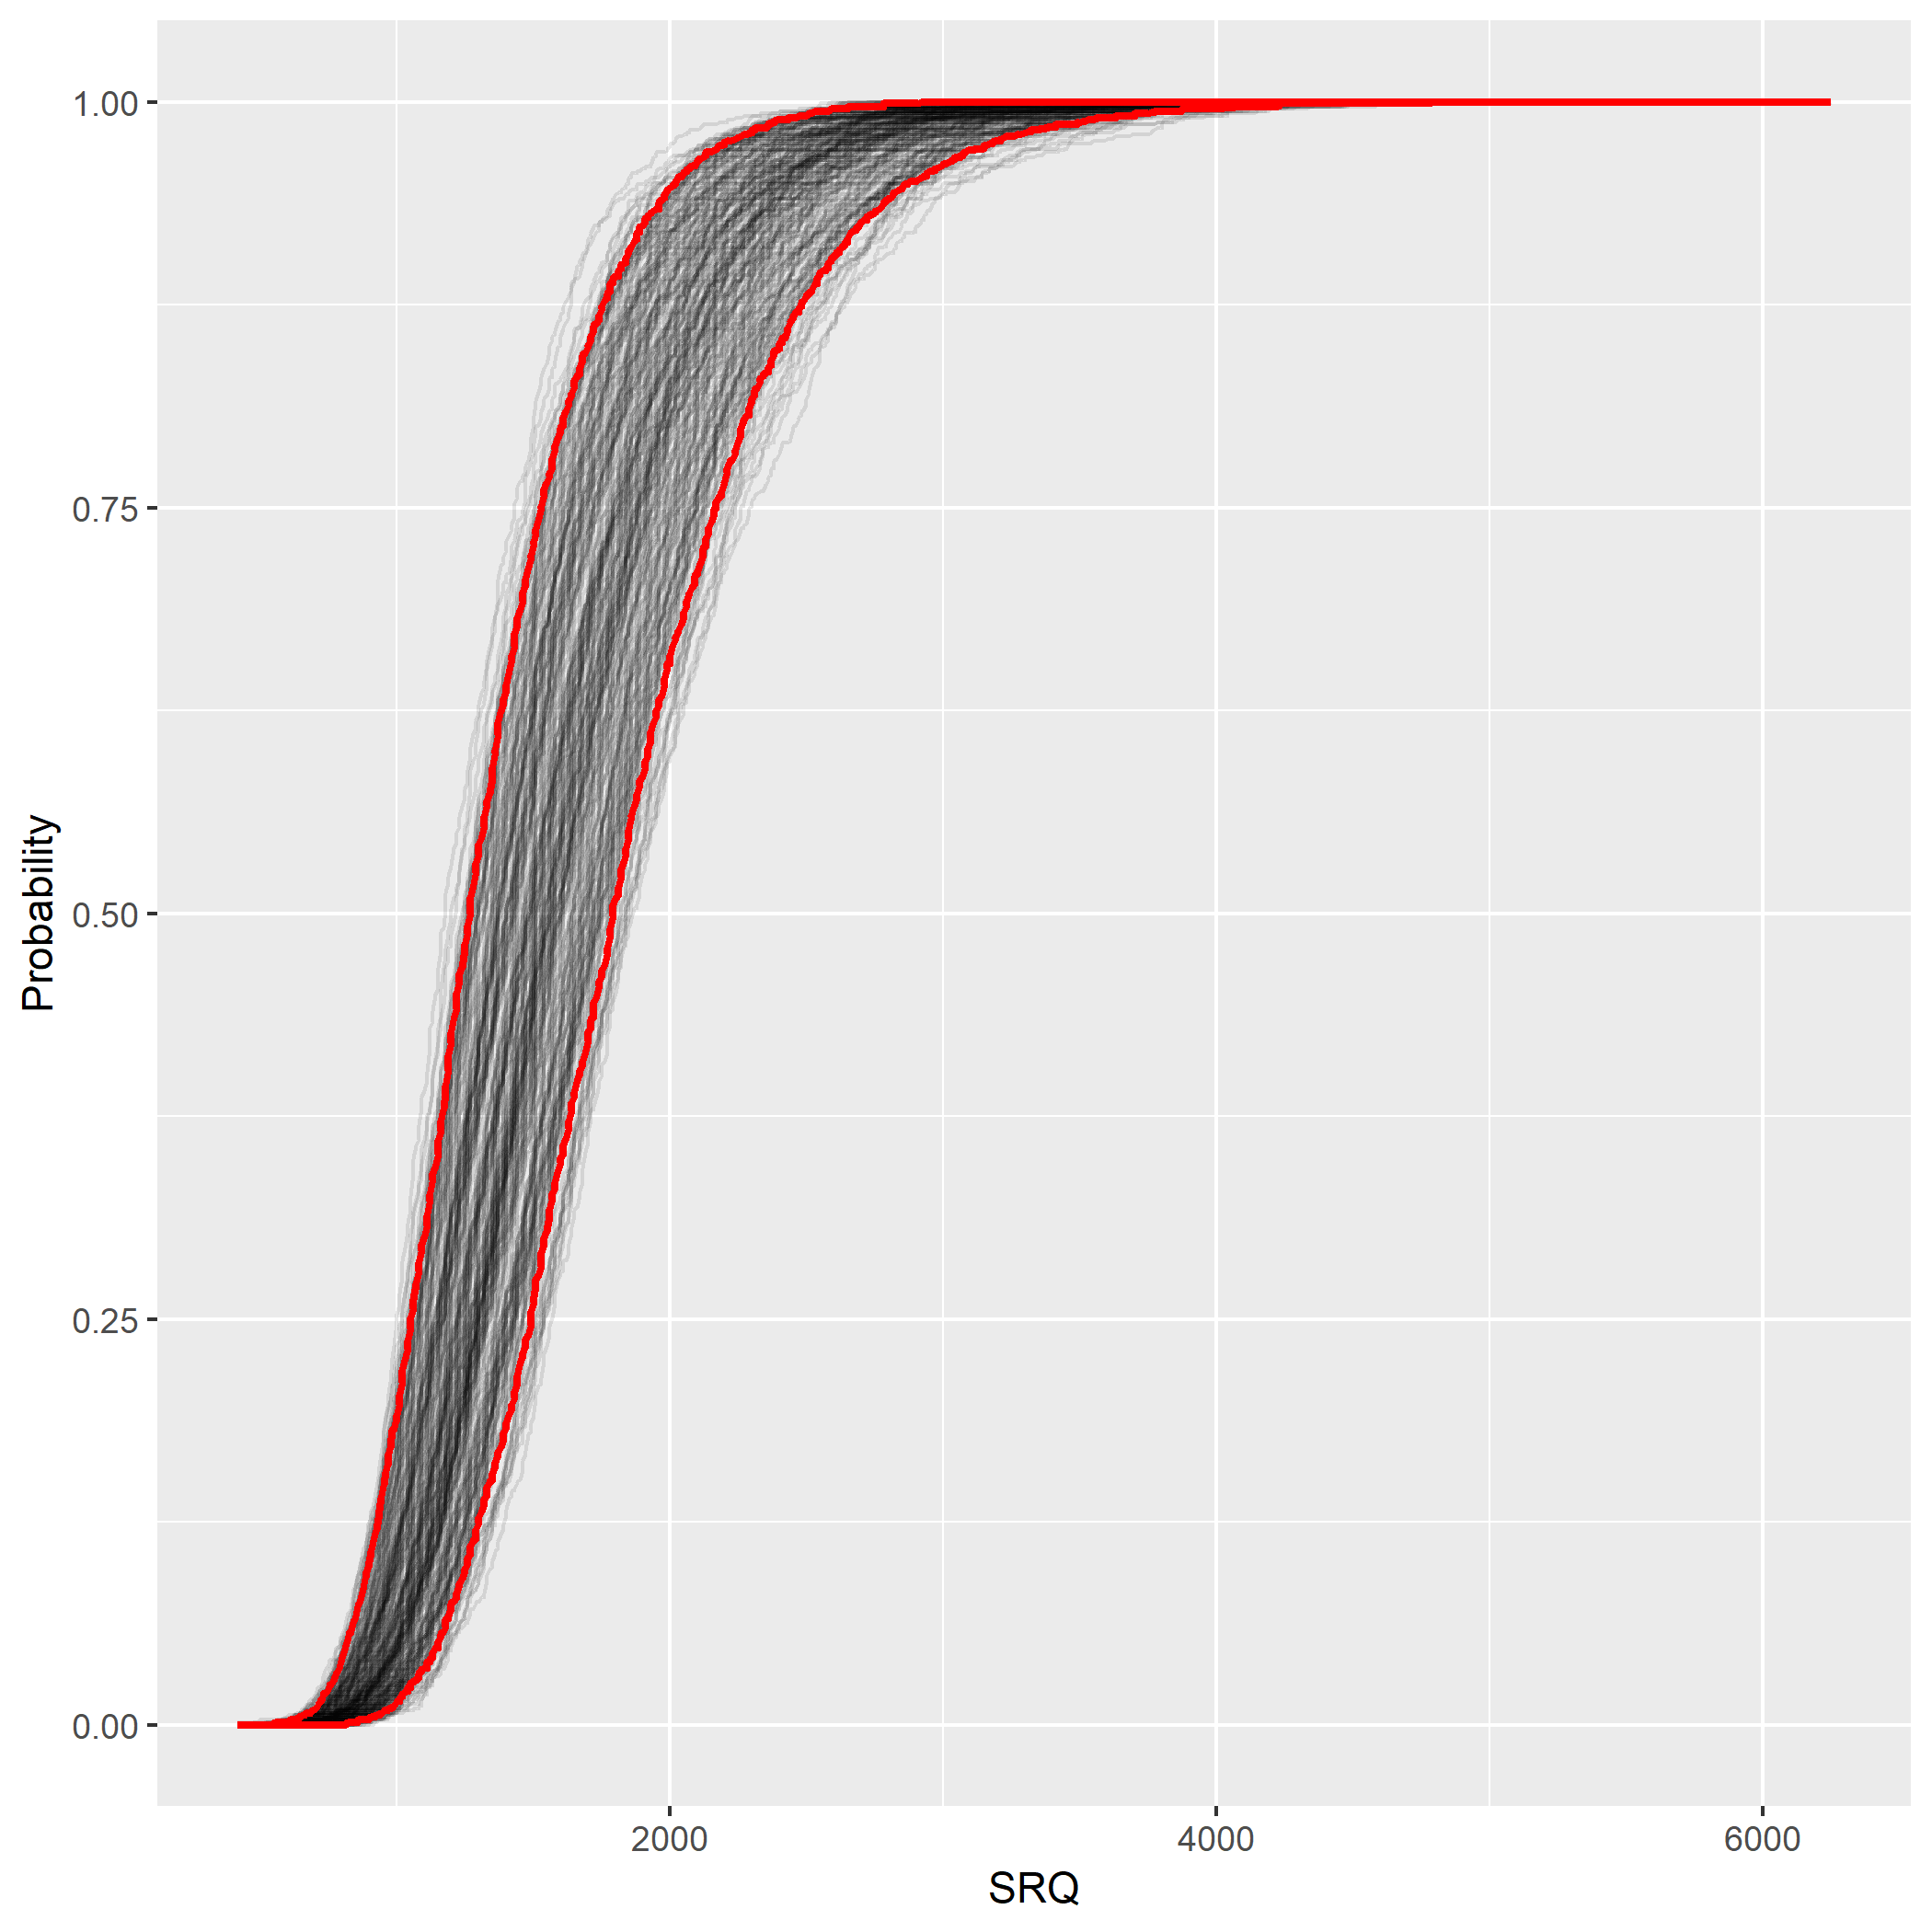
\includegraphics[height=4.3cm,width=4.3cm]{figures2/dwnld_plt.png} 
\end{center} 
\caption{\label{dwnld_plt}Plots downloaded and saved from the web application.}
\end{figure}

\begin{figure}[t]
\begin{center} 
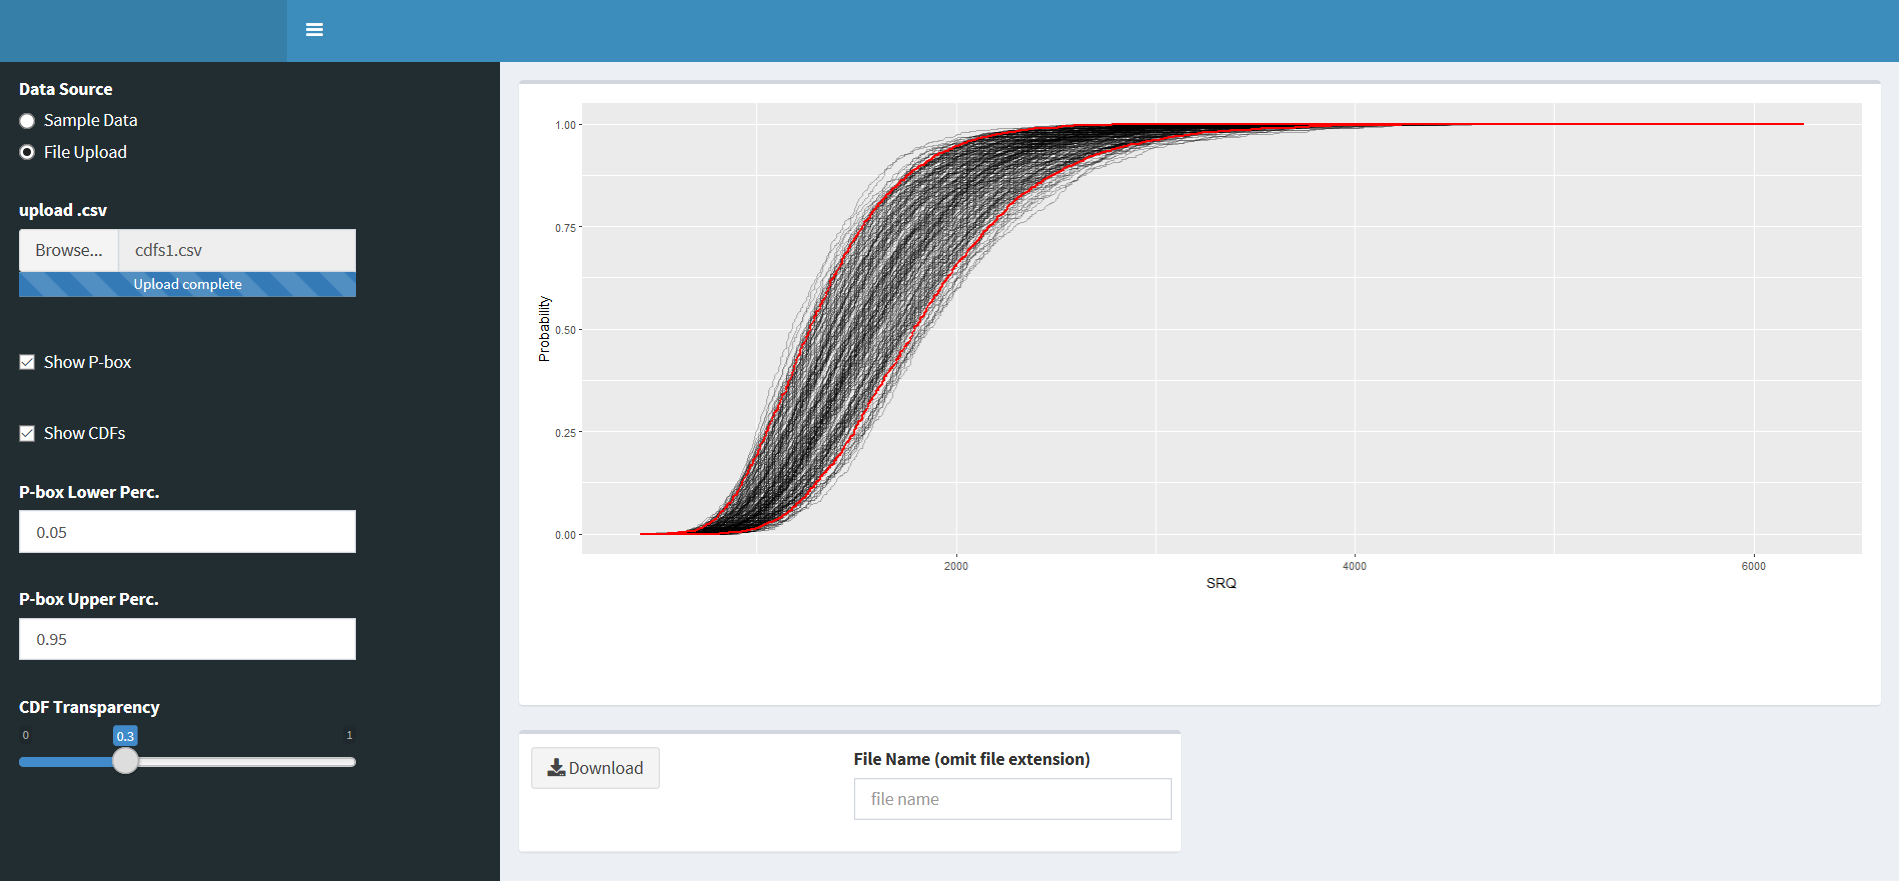
\includegraphics[height=8cm,width=15.5cm]{figures2/SS_full.png}
\end{center} 
\caption{\label{full}Full screenshot.}
\end{figure}

\subsection{Challenges}
One main challenge with this visualization tool that was unanticipated was the time that it would take to render the plot. The nature of uncertainty quantificataion and the nature of this kind of visualization leads to there being hundreds or even thousands of traces on a single plot. In addition, the way the {\tt shiny} package is implemented causes the plot to completely re-render when user inputs change. Thus, whenever the user selects a new plotting option, he or she must wait several seconds (depending on the size of the data set being used) for the plot to re-render. This leads to a less `interactive' feel for the user. As this application is still under development, possibilites for decreasing the re-rendering time of the plots are being explored. 

%%%%%%%%%%%%%%%%%%%%%%%%%
\section{Future Work}
\label{Future}
%%%%%%%%%%%%%%%%%%%%%%%%%

In the next two weeks I plan to fine-tune the visualization tool and produce a polished final product. There is also one more major feature to implement that will greatly aid in the interpretabilty of the visualization. This feature is the ability for a user to input an SRQ value and extract a probability range, as well as the ability to input a probability and extract an SRQ range. Finishing touches will also include adjusting the spacing between controls to improve aesthetics and adding a user manual/help page. 

%%%%%%%%%%%%%%%%%%%%%%%%%
\section{Appendix}
\label{Appendix}
%%%%%%%%%%%%%%%%%%%%%%%%%

{\tt R} code for {\tt shiny} web application.

\subsection{{\tt ui.R}}

%
\begin{knitrout}
\definecolor{shadecolor}{rgb}{0.969, 0.969, 0.969}\color{fgcolor}\begin{kframe}
\begin{alltt}
\hlkwd{library}\hlstd{(shiny)}
\hlkwd{library}\hlstd{(shinydashboard)}
\hlkwd{library}\hlstd{(plotly)}

\hlkwd{dashboardPage}\hlstd{(}
  \hlkwd{dashboardHeader}\hlstd{(),}
  \hlkwd{dashboardSidebar}\hlstd{(}
    \hlkwc{width} \hlstd{=} \hlnum{400}\hlstd{,}
    \hlkwd{radioButtons}\hlstd{(}\hlkwc{inputId} \hlstd{=} \hlstr{'radioDataSource'}\hlstd{,}
                 \hlkwc{label} \hlstd{=} \hlstr{'Data Source'}\hlstd{,}
                 \hlkwc{choices} \hlstd{=} \hlkwd{c}\hlstd{(}\hlstr{"Sample Data"}\hlstd{,}
                             \hlstr{"File Upload"}\hlstd{),}
                 \hlkwc{selected} \hlstd{=} \hlstr{"Sample Data"}\hlstd{),}
    \hlkwd{fileInput}\hlstd{(}\hlkwc{inputId} \hlstd{=} \hlstr{"fileIn"}\hlstd{,} \hlkwc{label} \hlstd{=} \hlstr{"upload .csv"}\hlstd{),}
    \hlkwd{checkboxInput}\hlstd{(}\hlkwc{inputId} \hlstd{=} \hlstr{"checkPbox"}\hlstd{,}
                  \hlkwc{label} \hlstd{=} \hlstr{"Show P-box"}\hlstd{,}
                  \hlkwc{value} \hlstd{=} \hlnum{TRUE}\hlstd{),}
    \hlkwd{checkboxInput}\hlstd{(}\hlkwc{inputId} \hlstd{=} \hlstr{"checkCDFs"}\hlstd{,}
                  \hlkwc{label} \hlstd{=} \hlstr{"Show CDFs"}\hlstd{,}
                  \hlkwc{value} \hlstd{=} \hlnum{TRUE}\hlstd{),}
    \hlkwd{numericInput}\hlstd{(}\hlkwc{inputId} \hlstd{=} \hlstr{"pboxLower"}\hlstd{,} \hlkwc{label} \hlstd{=} \hlstr{"P-box Lower Perc."}\hlstd{,}
                 \hlkwc{value} \hlstd{=} \hlnum{0.05}\hlstd{),}
    \hlkwd{numericInput}\hlstd{(}\hlkwc{inputId} \hlstd{=} \hlstr{"pboxUpper"}\hlstd{,} \hlkwc{label} \hlstd{=} \hlstr{"P-box Upper Perc."}\hlstd{,}
                 \hlkwc{value} \hlstd{=} \hlnum{0.95}\hlstd{),}
    \hlkwd{sliderInput}\hlstd{(}\hlkwc{inputId} \hlstd{=} \hlstr{"sliderAlpha"}\hlstd{,} \hlkwc{label} \hlstd{=} \hlstr{"CDF Transparency"}\hlstd{,}
                \hlkwc{value} \hlstd{=} \hlnum{0.3}\hlstd{,}
                \hlkwc{min} \hlstd{=} \hlnum{0}\hlstd{,}
                \hlkwc{max} \hlstd{=} \hlnum{1}\hlstd{,}
                \hlkwc{step} \hlstd{=} \hlnum{0.1}\hlstd{,}
                \hlkwc{ticks} \hlstd{=} \hlnum{FALSE}\hlstd{)}
  \hlstd{),}
  \hlkwd{dashboardBody}\hlstd{(}
    \hlkwd{fluidRow}\hlstd{(}
      \hlkwd{box}\hlstd{(}
        \hlkwc{width} \hlstd{=} \hlnum{12}\hlstd{,}
        \hlkwc{height} \hlstd{=} \hlnum{500}\hlstd{,}
        \hlcom{# main plot}
        \hlkwd{plotOutput}\hlstd{(}\hlstr{"uqPlot"}\hlstd{)}
      \hlstd{)}
    \hlstd{),}
    \hlkwd{fluidRow}\hlstd{(}
      \hlkwd{box}\hlstd{(}
        \hlkwd{splitLayout}\hlstd{(}
          \hlkwd{downloadButton}\hlstd{(}\hlkwc{outputId} \hlstd{=} \hlstr{'savePng'}\hlstd{),}
          \hlkwd{textInput}\hlstd{(}\hlkwc{inputId} \hlstd{=} \hlstr{"pngName"}\hlstd{,} \hlkwc{value} \hlstd{=} \hlstr{""}\hlstd{,} \hlkwc{placeholder} \hlstd{=} \hlstr{"file name"}\hlstd{,} \hlkwc{label} \hlstd{=} \hlstr{"File Name (omit file extension)"}\hlstd{)}
        \hlstd{)}
      \hlstd{)}
    \hlstd{)}
  \hlstd{)}
\hlstd{)}
\end{alltt}
\end{kframe}
\end{knitrout}

\subsection{{\tt server.R}}
%
\begin{knitrout}
\definecolor{shadecolor}{rgb}{0.969, 0.969, 0.969}\color{fgcolor}\begin{kframe}
\begin{alltt}
\hlcom{#}
\hlcom{# This is the server logic of a Shiny web application. You can run the }
\hlcom{# application by clicking 'Run App' above.}
\hlcom{#}
\hlcom{# Find out more about building applications with Shiny here:}
\hlcom{# }
\hlcom{#    http://shiny.rstudio.com/}
\hlcom{#}

\hlkwd{library}\hlstd{(shiny)}
\hlkwd{library}\hlstd{(ggplot2)}
\hlkwd{library}\hlstd{(plotly)}
\hlkwd{library}\hlstd{(dplyr)}

\hlcom{###############################################}
\hlcom{# Functions ###################################}
\hlcom{###############################################}
\hlstd{plotAllLayers} \hlkwb{<-} \hlkwa{function}\hlstd{(}\hlkwc{df}\hlstd{)\{}
  \hlstd{p}\hlkwb{<-}\hlkwd{ggplot}\hlstd{(}\hlkwc{data} \hlstd{= df,} \hlkwd{aes}\hlstd{(df[,}\hlnum{1}\hlstd{]))}
  \hlkwa{for}\hlstd{(i} \hlkwa{in} \hlkwd{names}\hlstd{(df)[}\hlopt{-}\hlnum{1}\hlstd{])\{}
    \hlstd{p}\hlkwb{<-}\hlstd{p}\hlopt{+}\hlkwd{geom_line}\hlstd{(}\hlkwd{aes_string}\hlstd{(}\hlkwc{y}\hlstd{=i),} \hlkwc{alpha} \hlstd{=} \hlnum{0.2}\hlstd{)}
  \hlstd{\}}
  \hlkwd{return}\hlstd{(p)}
\hlstd{\}}

\hlstd{calc_pbox} \hlkwb{<-} \hlkwa{function}\hlstd{(}\hlkwc{data}\hlstd{,} \hlkwc{p_upper}\hlstd{,} \hlkwc{p_lower}\hlstd{)\{}
  \hlcom{# for row in np.transpose(cdf_arr): # loop over transposed matrix}
  \hlcom{#   qlower = np.quantile(row, q = pbox_lower) # calculate lower quantile}
  \hlcom{#   qupper = np.quantile(row, q = pbox_upper) # calculate upper quantile}
  \hlcom{#   ql[counter] = qlower # store}
  \hlcom{#   qu[counter] = qupper # store}
  \hlcom{#   counter = counter + 1 }
  \hlstd{pbox} \hlkwb{<-} \hlkwd{apply}\hlstd{(values}\hlopt{$}\hlstd{data,} \hlnum{1}\hlstd{,} \hlkwc{FUN} \hlstd{= quantile,} \hlkwc{probs} \hlstd{=} \hlkwd{c}\hlstd{(p_lower, p_upper))}
  \hlcom{# pbox <- data_frame(pbox)}
  \hlkwd{return}\hlstd{(}\hlkwd{t}\hlstd{(pbox))}
\hlstd{\}}

\hlcom{###############################################}
\hlcom{# Reactive Values##############################}
\hlcom{###############################################}

\hlstd{values} \hlkwb{<-} \hlkwd{reactiveValues}\hlstd{()}

\hlcom{###############################################}
\hlcom{# Read in Sample Data #########################}
\hlcom{###############################################}
\hlstd{cdf_arr} \hlkwb{<-}  \hlkwd{read.csv}\hlstd{(}\hlstr{'data/cdfs.csv'}\hlstd{,} \hlkwc{header} \hlstd{=} \hlnum{FALSE}\hlstd{)}
\hlstd{cdf_arr} \hlkwb{<-}  \hlkwd{t}\hlstd{(cdf_arr)}
\hlstd{cdf_df} \hlkwb{<-}  \hlkwd{data.frame}\hlstd{(cdf_arr)}

\hlcom{###############################################}
\hlcom{# Server Logic ################################}
\hlcom{###############################################}
\hlkwd{shinyServer}\hlstd{(}\hlkwa{function}\hlstd{(}\hlkwc{input}\hlstd{,} \hlkwc{output}\hlstd{) \{}

  \hlstd{output}\hlopt{$}\hlstd{uqPlot} \hlkwb{<-} \hlkwd{renderPlot}\hlstd{(\{}
    \hlkwa{if}\hlstd{(input}\hlopt{$}\hlstd{radioDataSource} \hlopt{==} \hlstr{"Sample Data"}\hlstd{)\{}
      \hlstd{values}\hlopt{$}\hlstd{data} \hlkwb{<-} \hlstd{cdf_df}
    \hlstd{\}} \hlkwa{else} \hlstd{\{}
      \hlkwd{req}\hlstd{(input}\hlopt{$}\hlstd{fileIn)}
      \hlstd{df} \hlkwb{<-} \hlkwd{read.csv}\hlstd{(input}\hlopt{$}\hlstd{fileIn}\hlopt{$}\hlstd{datapath,}
                     \hlkwc{header} \hlstd{=} \hlnum{FALSE}\hlstd{)}
      \hlstd{df} \hlkwb{<-} \hlkwd{data.frame}\hlstd{(df)}
      \hlstd{values}\hlopt{$}\hlstd{data} \hlkwb{<-} \hlstd{df}
    \hlstd{\}}

    \hlkwd{req}\hlstd{(values}\hlopt{$}\hlstd{data)}
    \hlstd{plt} \hlkwb{<-} \hlkwd{ggplot}\hlstd{(}\hlkwc{data} \hlstd{= values}\hlopt{$}\hlstd{data,} \hlkwd{aes}\hlstd{(values}\hlopt{$}\hlstd{data[,}\hlnum{1}\hlstd{]))}
    \hlkwa{if}\hlstd{(input}\hlopt{$}\hlstd{checkCDFs} \hlopt{==} \hlnum{TRUE}\hlstd{)\{}
      \hlkwa{for}\hlstd{(i} \hlkwa{in} \hlkwd{names}\hlstd{(values}\hlopt{$}\hlstd{data)[}\hlopt{-}\hlnum{1}\hlstd{])\{}
        \hlstd{plt} \hlkwb{<-} \hlstd{plt} \hlopt{+} \hlkwd{geom_line}\hlstd{(}\hlkwd{aes_string}\hlstd{(}\hlkwc{y}\hlstd{=i),} \hlkwc{alpha} \hlstd{= input}\hlopt{$}\hlstd{sliderAlpha)}
      \hlstd{\}}
    \hlstd{\}}
    \hlstd{plt} \hlkwb{<-} \hlstd{plt} \hlopt{+}
      \hlkwd{xlab}\hlstd{(}\hlstr{"SRQ"}\hlstd{)} \hlopt{+}
      \hlkwd{ylab}\hlstd{(}\hlstr{"Probability"}\hlstd{)}

    \hlkwa{if}\hlstd{(input}\hlopt{$}\hlstd{checkPbox} \hlopt{==} \hlnum{TRUE}\hlstd{)\{}
      \hlstd{pbox} \hlkwb{<-} \hlkwd{calc_pbox}\hlstd{(values}\hlopt{$}\hlstd{data, (}\hlnum{1} \hlopt{-} \hlstd{input}\hlopt{$}\hlstd{pboxLower), (}\hlnum{1} \hlopt{-} \hlstd{input}\hlopt{$}\hlstd{pboxUpper))}
      \hlstd{plt} \hlkwb{<-} \hlstd{plt} \hlopt{+}
        \hlkwd{geom_line}\hlstd{(}\hlkwd{aes}\hlstd{(}\hlkwc{y} \hlstd{= pbox[,}\hlnum{1}\hlstd{]),} \hlkwc{col} \hlstd{=} \hlstr{"red"}\hlstd{,} \hlkwc{lwd} \hlstd{=} \hlnum{1}\hlstd{)} \hlopt{+}
        \hlkwd{geom_line}\hlstd{(}\hlkwd{aes}\hlstd{(}\hlkwc{y} \hlstd{= pbox[,}\hlnum{2}\hlstd{]),} \hlkwc{col} \hlstd{=} \hlstr{"red"}\hlstd{,} \hlkwc{lwd} \hlstd{=} \hlnum{1}\hlstd{)}
    \hlstd{\}}

    \hlstd{values}\hlopt{$}\hlstd{plot} \hlkwb{<-} \hlstd{plt}

    \hlstd{plt}
  \hlstd{\})}

  \hlcom{# help from https://stackoverflow.com/questions/14810409/save-plots-made-in-a-shiny-app}
  \hlstd{output}\hlopt{$}\hlstd{savePng} \hlkwb{<-} \hlkwd{downloadHandler}\hlstd{(}
    \hlkwc{filename} \hlstd{=} \hlkwa{function}\hlstd{() \{} \hlkwd{paste}\hlstd{(input}\hlopt{$}\hlstd{pngName,} \hlstr{'.png'}\hlstd{,} \hlkwc{sep}\hlstd{=}\hlstr{''}\hlstd{) \},}
    \hlkwc{content} \hlstd{=} \hlkwa{function}\hlstd{(}\hlkwc{file}\hlstd{) \{}
      \hlkwd{ggsave}\hlstd{(file,} \hlkwc{plot} \hlstd{= values}\hlopt{$}\hlstd{plot,} \hlkwc{device} \hlstd{=} \hlstr{"png"}\hlstd{)}
    \hlstd{\}}
  \hlstd{)}

\hlstd{\})}
\end{alltt}
\end{kframe}
\end{knitrout}

\newpage

\bibliographystyle{elsarticle-harv}
% modified to add 
%     \itemsep=0pt
% to 2nd line of file paper.bbl

\bibliography{references2}

\end{document}
